\begin{figure}[h]
	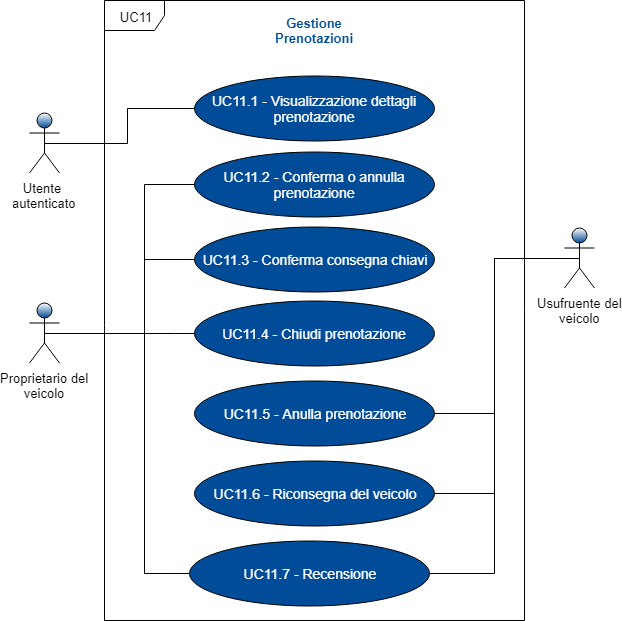
\includegraphics[width=12cm]{res/images/UC12Prenotazioni.png}
	\centering
	\caption{UC11 - Gestione prenotazioni}
\end{figure}
\subsubsection{UC11 - Gestione prenotazioni}
\begin{itemize}
	\item \textbf{Attori Primari}: utente autenticato;
	\item \textbf{Attori Secondari}:
	usufruente del veicolo, proprietario del veicolo;
	\item \textbf{Descrizione}: agli utenti autenticati è resa disponibile una maschera che presenta la lista di tutte le sue prenotazioni ancora attive, dalla quale l'utente può scegliere di effettuare operazioni di gestione su ognuna di esse;
	per ogni prenotazione presente nella lista saranno visualizzati dei dettagli riassuntivi, che sono:
	\begin{itemize}
		\item marca del veicolo prenotato;
		\item modello del veicolo prenotato;
		\item stato della prenotazione:
		\item data;
		\item fascia oraria;
		\item immagine del veicolo.
	\end{itemize}
	\item \textbf{Scenario principale}: l'utente autenticato effettua operazioni di gestione di una prenotazione. Esse comprendono:
	\begin{itemize}
		\item visualizzazione dettagli prenotazione [UC11.1].
	\end{itemize}
	\item \textbf{Scenario alternativo}: Se l'utente autenticato è il proprietario del veicolo, inoltre può:
	\begin{itemize}
		\item confermare o annullare le prenotazioni ricevute [UC11.2];
		\item confermare la consegna delle chiavi [UC11.3]
		\item confermare la riconsegna del veicolo [UC11.4];
		\item recensire l'usufruente [UC11.7].
	\end{itemize}
	Se l'utente autenticato è l'usufruente del veicolo, inoltre potrà:
	\begin{itemize}
		\item annullare la prenotazione [UC11.5];
		\item richiedere la conferma della riconsegna del veicolo [UC11.6];
		\item recensire il proprietario [UC11.7].
	\end{itemize}
	\item \textbf{Precondizione}: il sistema carica correttamente la lista delle prenotazioni effettuate attualmente attive;
	\item \textbf{Postcondizione}: l'utente ha visualizzato le sue prenotazioni correnti ed è riuscito ad effettuare eventuali modifiche.
\end{itemize} 
 \subsubsection{UC11.1 - Visualizzazione dettagli prenotazione}
\begin{itemize}
	\item \textbf{Attori Primari}: utente autenticato;
	\item \textbf{Descrizione}: l'utente visualizza i dettagli della prenotazione scelta dalla maschera di presentazione delle prenotazioni, ciò gli permette di visualizzare:
	\begin{itemize}
		%\item nome del proprietario del veicolo o dell'usufruente;
		\item la marca del veicolo prenotato;
		\item il modello del veicolo prenotato;
		\item lo stato della prenotazione
		\item la data;
		\item la fascia oraria.	
		\item il luogo d'incontro;
	\end{itemize}
	\item \textbf{Scenario principale}: l'utente visualizza i dettagli della prenotazione;	
	\item \textbf{Precondizione}: l'utente ha scelto una prenotazione;
	\item \textbf{Postcondizione}: l'utente ha visualizzato correttamente i dettagli della prenotazione.
\end{itemize}
\subsubsection{UC11.2 - Conferma o annulla prenotazione}
\begin{itemize}
	\item \textbf{Attori Primari}: proprietario del veicolo;
	\item \textbf{Descrizione}: il proprietario del veicolo conferma o annulla la richiesta di prenotazione ricevuta;
	\item \textbf{Scenario principale}: l'utente si trova all'interno della pagina di visualizzazione dei dettagli della richiesta di prenotazione appena ricevuta. Se conferma allora verrà inserito, nella prenotazione, il luogo d'incontro che è la posizione della macchina indicata nel momento in cui il proprietario ha aggiunto il veicolo.\newline
	Se annulla, la prenotazione verrà chiusa e cancellata;
	\item \textbf{Precondizione}: l'utente visualizza correttamente la prenotazione che intende confermare o annullare;
	\item \textbf{Postcondizione}: l'utente ha confermato o annullato correttamente la richiesta di prenotazione ricevuta.
\end{itemize}
\subsubsection{UC11.3 - Conferma consegna chiavi}
\begin{itemize}
	\item \textbf{Attori Primari}: proprietario del veicolo;
	\item \textbf{Descrizione}: il proprietario del veicolo conferma, tramite l'apposito pulsante, che le chiavi sono state consegnate all'usufruente del veicolo;
	\item \textbf{Scenario principale}: l'utente si trova all'interno della pagina di visualizzazione dei dettagli della richiesta di prenotazione appena ricevuta. In quanto confermata, viene reso disponibile la conferma della consegna delle chiavi del veicolo all'usufruente;
	\item \textbf{Precondizione}: l'utente visualizza correttamente la prenotazione e intende confermare la consegna delle chiavi del veicolo;
	\item \textbf{Postcondizione}: l'utente ha confermato la consegna delle chiavi del veicolo all'usufruente.
\end{itemize}
\subsubsection{UC11.4 - Chiudi prenotazione}
\begin{itemize}
	\item \textbf{Attori Primari}: proprietario del veicolo;
	\item \textbf{Descrizione}: il proprietario del veicolo conferma la riconsegna del mezzo e delle chiavi e chiude definitivamente la prenotazione;
	\item \textbf{Scenario principale}: l'utente si trova all'interno della pagina di visualizzazione dei dettagli della prenotazione precedentemente selezionata. Alla riconsegna del veicolo e delle chiavi, attraverso l'apposito pulsante l'utente confermerà la chiusura della prenotazione in modo definitivo. Comparirà un pop-up che permetterà di lasciare una recensione all'altro utente [UC11.7];
	\item \textbf{Precondizione}: l'utente visualizza correttamente la prenotazione che intende concludere;
	\item \textbf{Postcondizione}: l'utente ha concluso correttamente la prenotazione selezionata.
\end{itemize}
\subsubsection{UC11.5 - Annulla prenotazione}
\begin{itemize}
	\item \textbf{Attori Primari}: usufruente del veicolo;
	\item \textbf{Descrizione}: l'utente usufruente potrà annullare la prenotazione selezionata qualora sia in attesa di conferma da parte del proprietario del veicolo;
	\item \textbf{Scenario principale}: l'utente si trova all'interno della pagina di visualizzazione dei dettagli della prenotazione precedentemente selezionata. Attraverso l'apposito pulsante l'utente cancellerà la prenotazione effettuata;
	\item \textbf{Precondizione}: l'utente ha premuto il pulsante per la cancellazione delle prenotazione precedentemente selezionata;
	\item \textbf{Postcondizione}: l'utente ha annullato correttamente la prenotazione selezionata.
\end{itemize}
\subsubsection{UC11.6 - Riconsegna del veicolo}
\begin{itemize}
	\item \textbf{Attori Primari}: usufruente del veicolo;
	\item \textbf{Descrizione}: l'utente, passato il tempo in cui ha prenotato il veicolo può chiudere la prenotazione e riconsegnare il mezzo al proprietario;
	\item \textbf{Scenario principale}: l'utente si trova all'interno della pagina di visualizzazione dei dettagli della prenotazione precedentemente selezionata. Dopo aver riconsegnato il veicolo e le chiavi, attraverso l'apposito pulsante l'utente chiederà la chiusura della prenotazione (la prenotazione verrà definitivamente chiusa quando anche il proprietario del veicolo confermerà la riconsegna delle chiavi e del mezzo [UC11.4]). Comparirà un pop-up che permetterà di lasciare una recensione all'altro utente [UC11.7];
	\item \textbf{Precondizione}: l'utente visualizza correttamente la prenotazione che intende concludere;
	\item \textbf{Postcondizione}: l'utente ha richiesto correttamente la chiusura della prenotazione selezionata.
\end{itemize}
\subsubsection{UC11.7 - Recensione}
\begin{itemize}
	\item \textbf{Attori Primari}: utente autenticato;
	\item \textbf{Descrizione}: l'utente recensisce l'altro utente coinvolto nella prenotazione;
	\item \textbf{Scenario principale}: l'utente visualizza il pop-up per inserire la recensione che consiste in una valutazione da una a cinque stelle;
	\item \textbf{Precondizione}: l'utente visualizza correttamente il pop-up;
	\item \textbf{Postcondizione}: l'utente ha inserito correttamente la recensione.
\end{itemize}

